\begin{tikzpicture}
        \node (A) at (0,0) {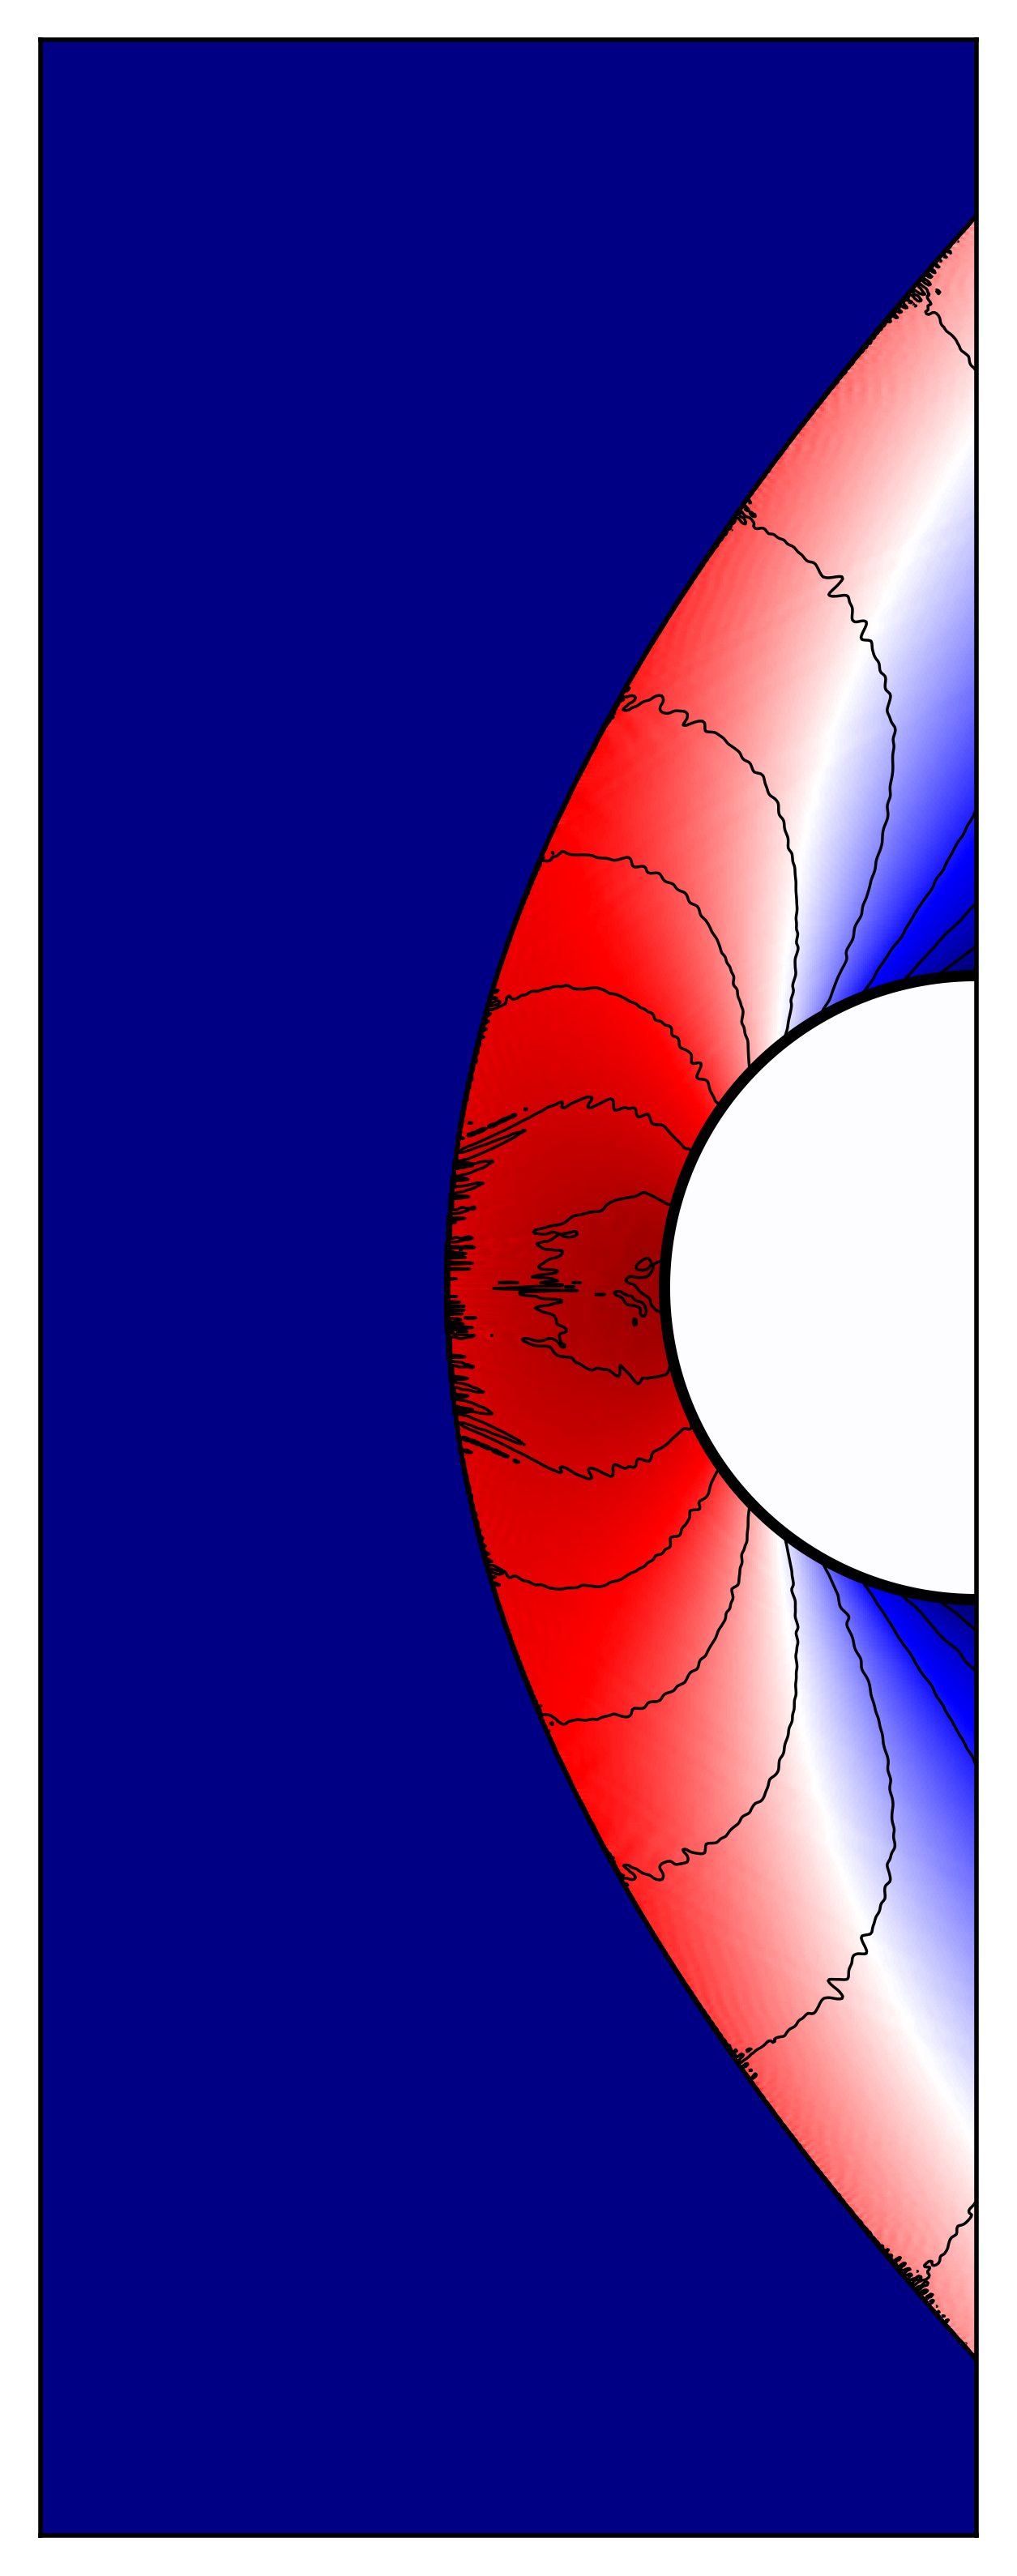
\includegraphics[scale=0.4]{imgs/bowshock_density_3.png}};
        \node [right = 0cm of A] (B) {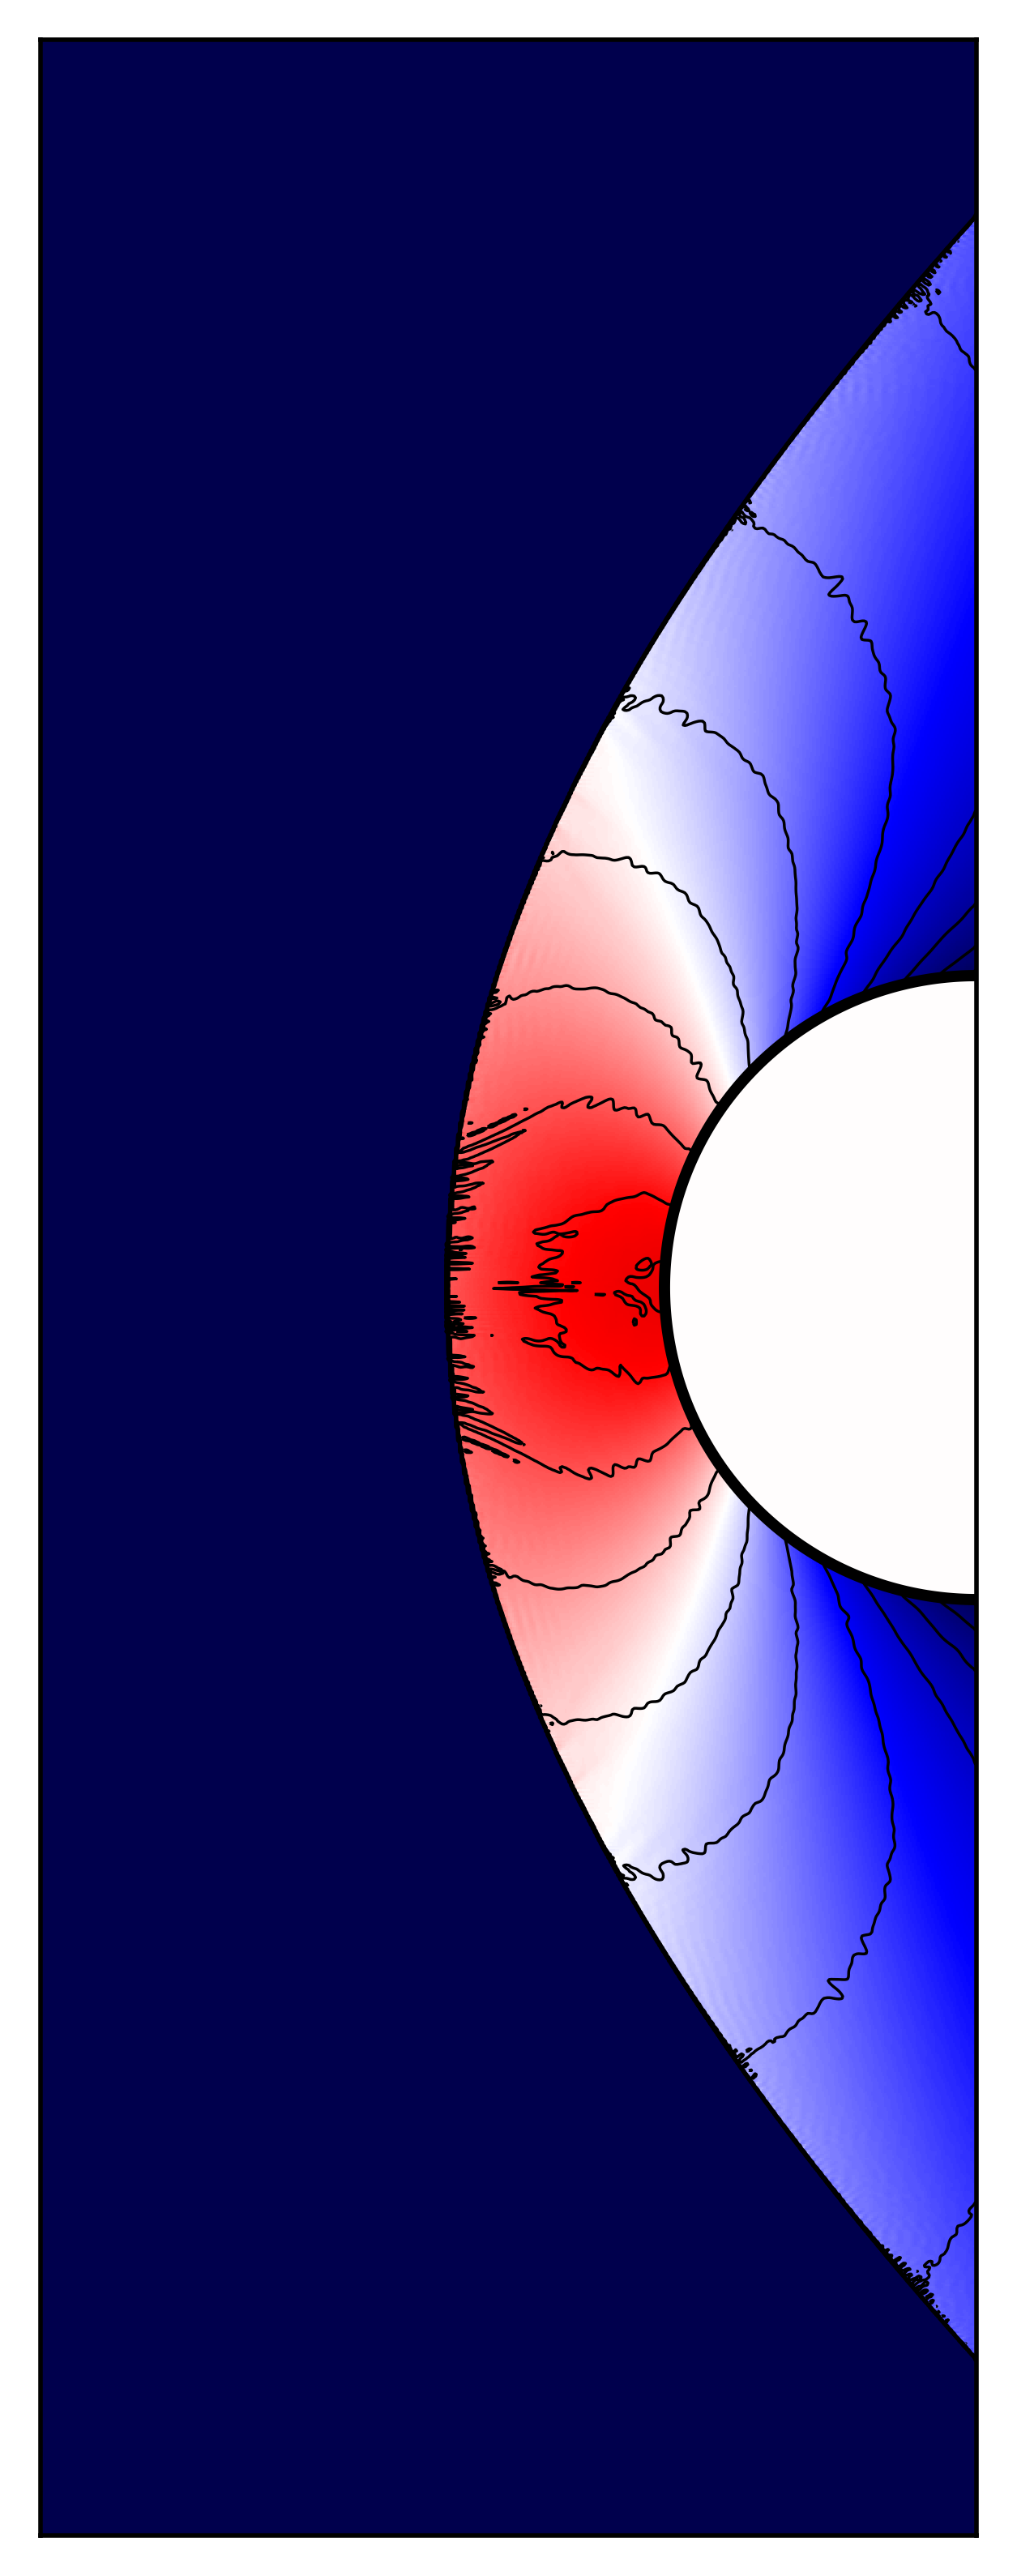
\includegraphics[scale=0.4]{imgs/bowshock_pressure_3.png}};
        \node at (A.north) {$\rho$};
        \node at (B.north) {$p$};
        \draw[->] ([xshift=-.1cm, yshift=-.2cm]A.south west) -- ([yshift=-.2cm, xshift=.4cm]A.south west) node[at end, below] {$x$};
        \draw[->] ([xshift=-.1cm, yshift=-.2cm]A.south west) -- ([yshift=.3cm, xshift=-.1cm]A.south west) node[at end, left] {$y$};

        \node [right = 2cm of B] (C)  {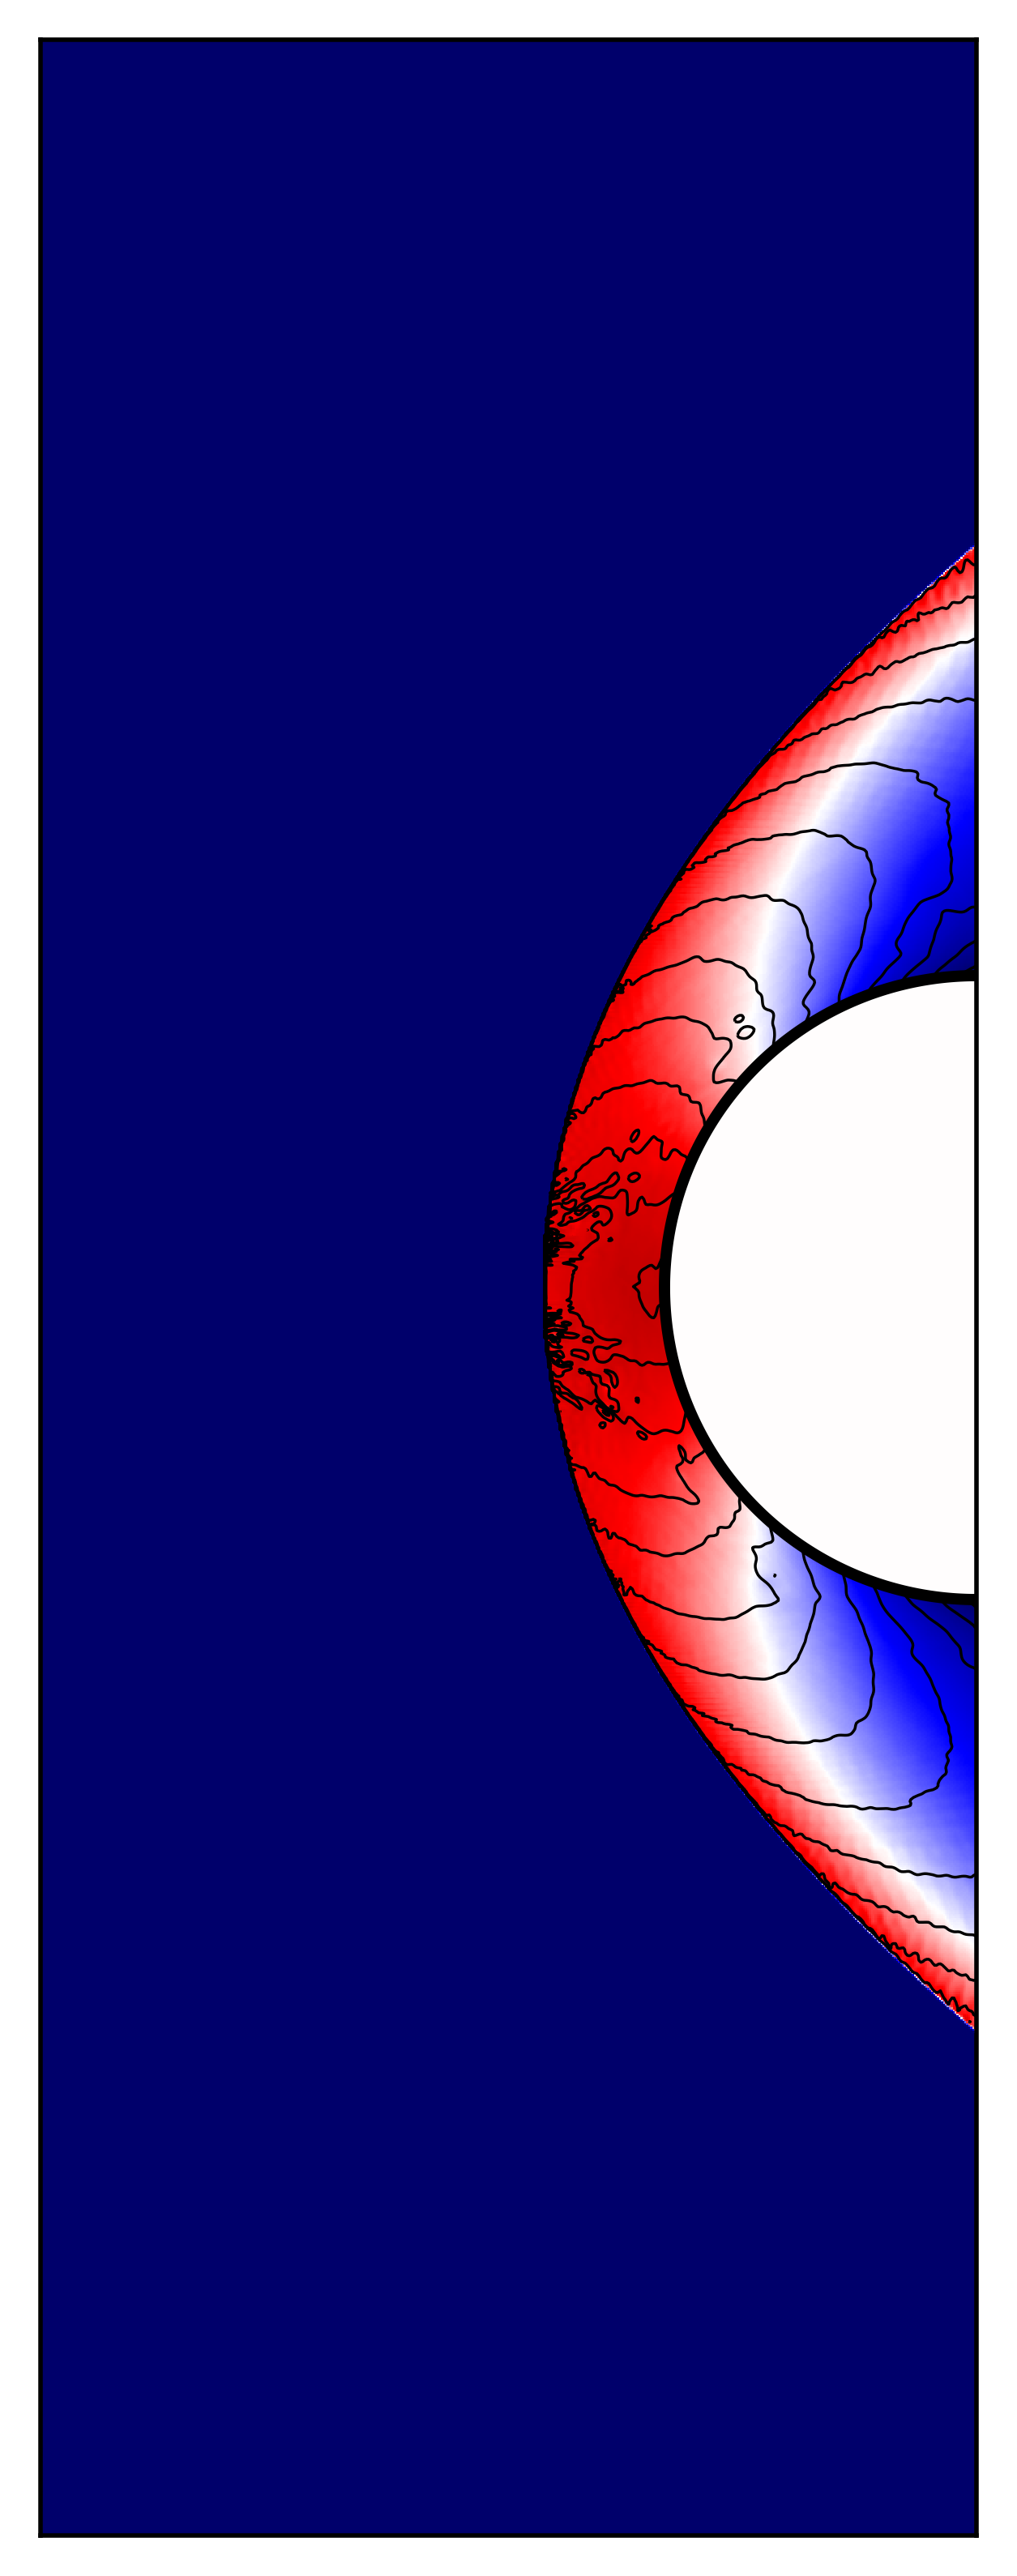
\includegraphics[scale=0.4]{imgs/bowshock_density_20.png}};
        \node [right = 0cm of C] (D) {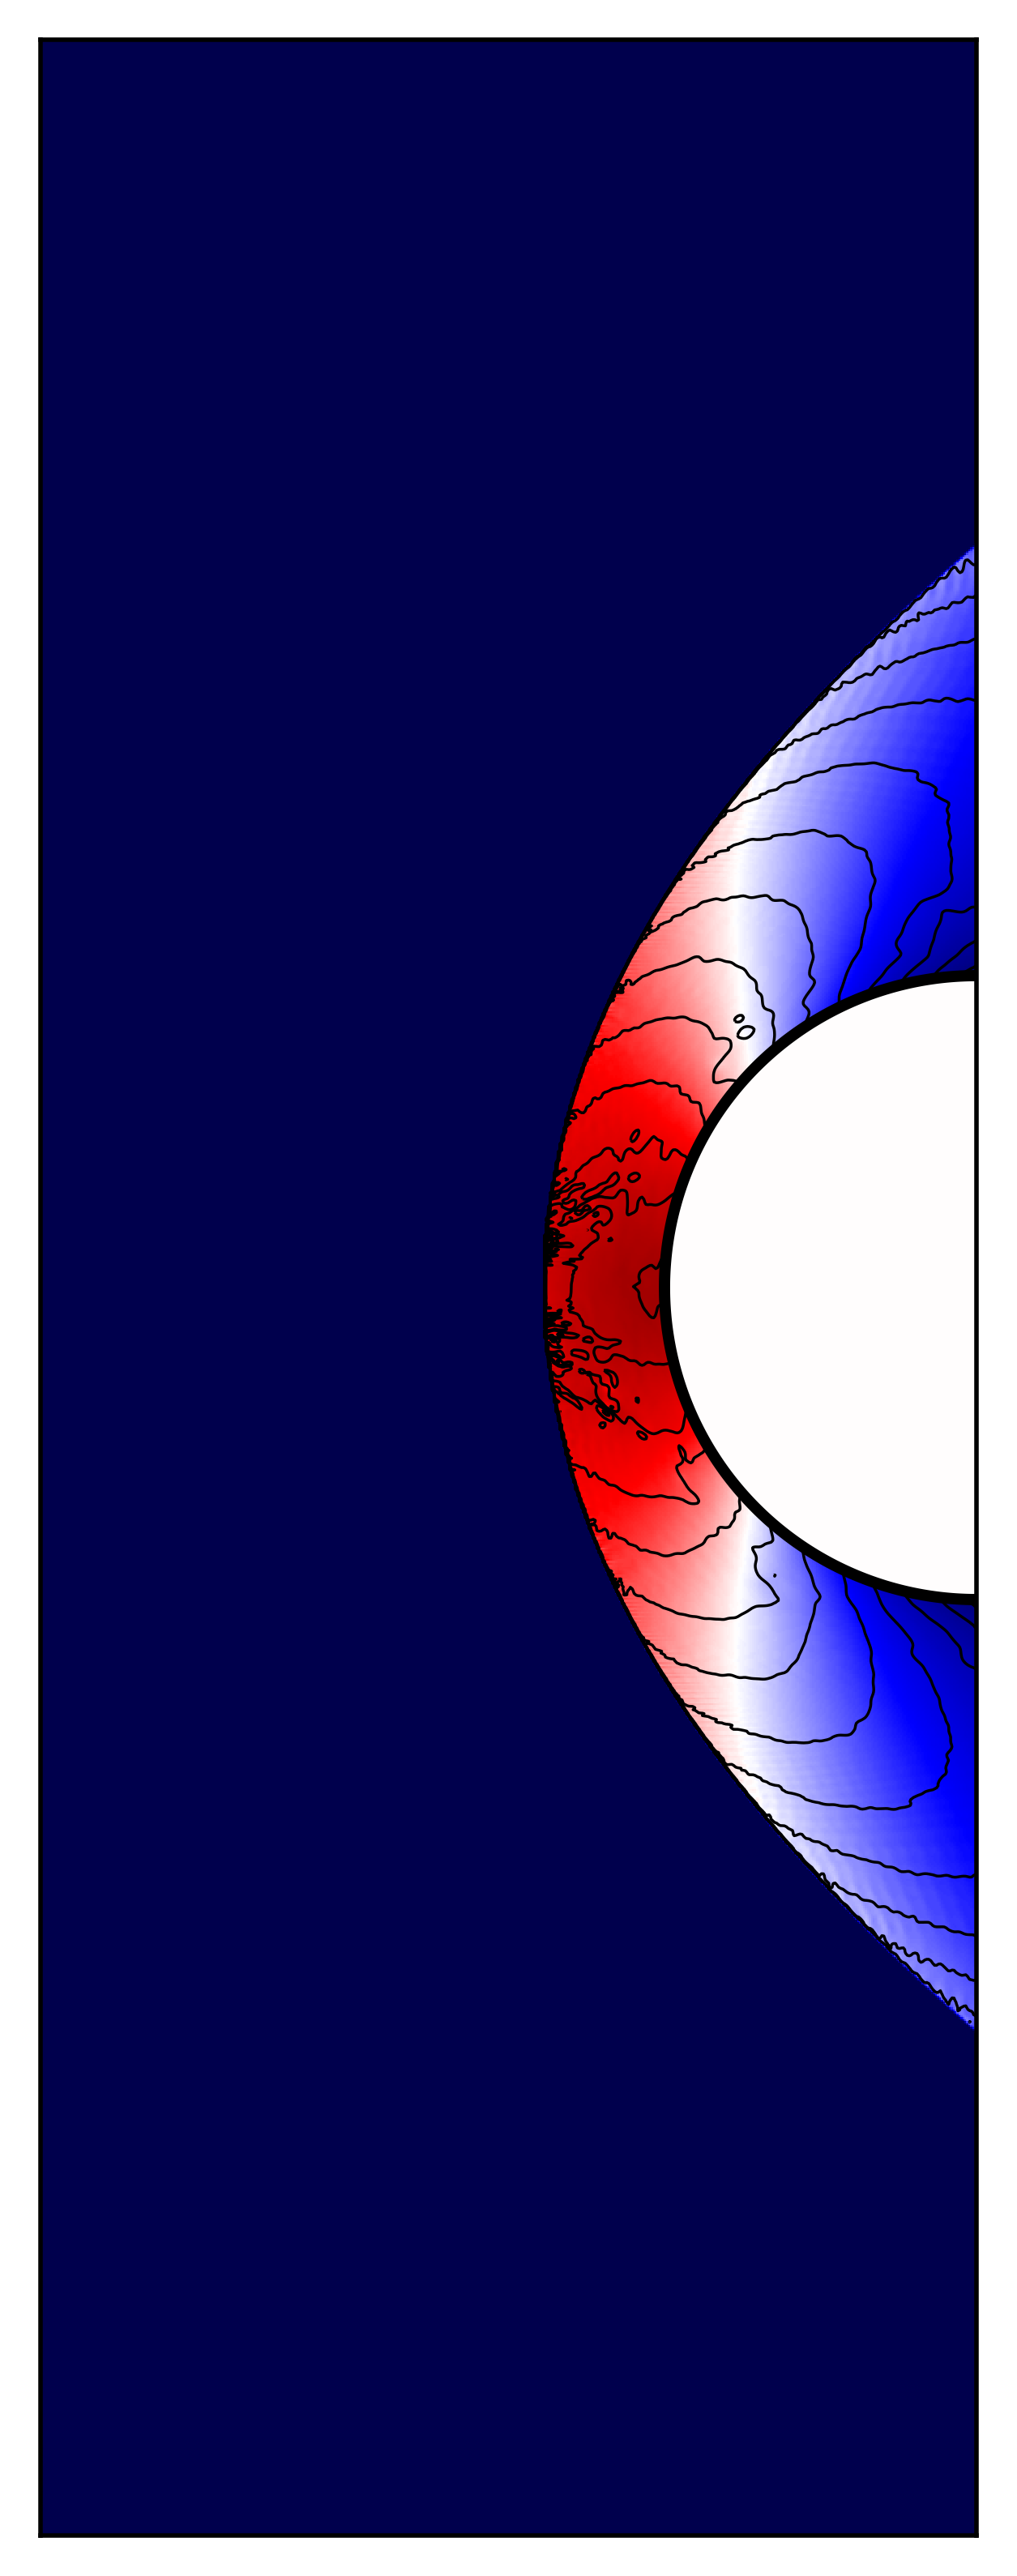
\includegraphics[scale=0.4]{imgs/bowshock_pressure_20.png}};
        \node at (C.north) {$\rho$};
        \node at (D.north) {$p$};
    \end{tikzpicture}